\documentclass{beamer}
\usepackage{moreverb} 
\usepackage{listings}
\usepackage{mflogo}
% imprimir
% \documentclass[handout]{beamer} 
% \usepackage{pgfpages}
% \pgfpagesuselayout{4 on 1}[a4paper,landscape,border shrink=5mm]

\mode<presentation> {
  \usetheme{Warsaw}
  \setbeamercovered{opaque}
}

\usebackgroundtemplate{
\includegraphics[width=\paperwidth]{format/libresoft-bg.png}}
% \usepackage[spanish]{babel}
\usepackage[utf8]{inputenc}
\usepackage{graphics}
\usepackage{amssymb} % Simbolos matematicos

%% Metadatos del PDF.
\hypersetup{  
  pdftitle={System Integration},
  pdfauthor={Miguel Vidal},
  pdfcreator={GSyC/Libresoft},
  pdfproducer=PDFLaTeX,
  pdfsubject={Master on Free Software},
}
%%

\defbeamertemplate*{footline}{shadow theme}
{%
  \leavevmode%
  \hbox{\begin{beamercolorbox}[wd=.5\paperwidth,ht=2.5ex,dp=1.125ex,leftskip=.1cm plus1fil,rightskip=.2cm]{author in head/foot}%

\includegraphics[scale=0.40]{format/cc-by-80x15.png} \hspace{0.05cm}
	Miguel Vidal / Jose Castro
  \end{beamercolorbox}%
  \begin{beamercolorbox}[wd=.5\paperwidth,ht=2.5ex,dp=1.125ex,leftskip=.3cm,rightskip=.3cm plus1fil]{title in head/foot}%
    \usebeamerfont{title in head/foot}\insertshorttitle%
    \hspace{.25cm} \usebeamerfont{author in head/foot}\insertframenumber\,/\,\inserttotalframenumber\hfill
  \end{beamercolorbox}}%
  \vskip0pt%
}


\begin{document}

\title{Introduction to System Administration with FOSS}
\subtitle{System Integration}
% \institute{\texttt{http://gsyc.urjc.es/\~{}mvidal} \\ Twitter: \texttt{@mvidallopez}}
\author{Miguel Vidal, Jose Castro} 
\date{\footnotesize{Master on Free Software \\ March 23rd, 2012}}
\author{Miguel Vidal \hspace{1cm} Jose Castro \\
\hspace{0.5mm} {\tiny Twitter: @mvidallopez \hspace{1.1cm}Twitter: @jfcastroluis}
}


\frame{
\maketitle
\begin{center}

\includegraphics[width=6cm]{format/gsyc-urjc}
\end{center}
}

%% License slide
\begin{frame}
  \vspace{2cm}
  \begin{flushright}
    {\small \copyright{} 2010-2012 Miguel Vidal, Jose Castro} \\
%    \vspace{0.25cm}
    \medskip
    {\scriptsize This work is licensed under \\ a Creative Commons Attribution 3.0 License}
%    \vspace{0.10cm}
  \end{flushright}
  \begin{flushright}
    \href{http://creativecommons.org/licenses/by/3.0/es}{
\includegraphics[width=2cm]{format/cc-by.png}} \\
    {\tiny \url{http://creativecommons.org/licenses/by/3.0}}
  \end{flushright}
\end{frame}%%

\usebackgroundtemplate{}

\AtBeginSection[]
{
\begin{frame}<beamer>
\begin{center}
{\huge \insertsection}
\end{center}
\end{frame}
}


\AtBeginSubsection[]
{
  \begin{frame}<beamer>{Índice}
    \tableofcontents[currentsection,currentsubsection]
  \end{frame}
}

%%

\normalsize



%%---------------------------------------------------------------------
%%---------------------------------------------------------------------

%%%%%%%%%%%%%%%%%%%%%%%%%%%%%%%%%%%%%%%%%%%%%%%%%%%%%%%%%%%%%%%%%%%%%%%
\section{El software libre en servidores}
%%%%%%%%%%%%%%%%%%%%%%%%%%%%%%%%%%%%%%%%%%%%%%%%%%%%%%%%%%%%%%%%%%%%%%%

\subsection{Ventajas del software libre en servidores}
\begin{frame}
\frametitle{Ventajas del software libre en servidores}

\begin{itemize}
\item Libertad de uso, modificación y redistribución: 
	\begin{itemize}
	\item podemos \alert{instalarlo} en tantas máquinas como queramos.
	\item podemos \alert{adaptarlo} a nuestras necesidades o las del cliente.
	\item podemos revisar el código y \alert{corregir} errores sin esperar a que lo haga el fabricante.
	\item podemos beneficiarnos de las mejoras y correcciones que hagan otros.
	\end{itemize}

\item  Corrección mas rápida y eficiente de fallos, y rápida resolución de dudas y problemas, gracias al \alert{modelo bazar} y a las fuertes comunidades que tiene detrás.

\end{itemize}
\end{frame}

%%%%%%%%%%%%%%%%%%%%%%%%%%%%%%%%%%%%%%%%%%%%%%%%%%%%%%%%%%%%%%%%%%%%%%%

\begin{frame}
\frametitle{Ventajas del software libre en servidores}

\begin{itemize}
\item \alert{Independencia tecnológica}: no nos atamos a ningún proveedor en particular.
\item Soporte y \alert{compatibilidad} a largo plazo: el fabricante no está forzado a ``vendernos'' continuamente nuevas versiones. 
\item Fomento de la \alert{libre competencia} al basarse en servicios y no en licencias.
\end{itemize}
\end{frame}

%%%%%%%%%%%%%%%%%%%%%%%%%%%%%%%%%%%%%%%%%%%%%%%%%%%%%%%%%%%%%%%%%%%%%%%

\begin{frame}
\frametitle{Ventajas del software libre en servidores}

\begin{itemize}
\item Ausencia de secretismo tecnológico y de patentes (seguridad jurídica). 
\item \alert{Formatos estándar}: facilitan la interoperabilidad y evitan incompatibilidades. 
\item Métodos simples y unificados de gestión de software: las distribuciones evitan tener que acudir a buscar software de fuentes dudosas.
\end{itemize}
\end{frame}

%%%%%%%%%%%%%%%%%%%%%%%%%%%%%%%%%%%%%%%%%%%%%%%%%%%%%%%%%%%%%%%%%%%%%%%

\begin{frame}
\frametitle{Ventajas del software libre en servidores}

\begin{itemize}
\item Inmensa \alert{variedad} de soluciones muy \alert{maduras}: el software libre nace en entornos de servidores.
\item Demanda de técnicos FLOSS en expansión, gracias a la creciente adopción por parte de las AA.PP. y de grandes empresas tecnológicas (Google, IBM, Sun/Oracle, etc.).
\item Sistemas \alert{potencialmente más seguros}: hackers y empresas de seguridad de todo el mundo puedan auditar los programas.
\item Aspectos económicos: más de mil millones de euros en licencias de Microsoft en España anuales (2006). Bajo TCO.
\item Fiabilidad y rendimiento.
\end{itemize}
\end{frame}

%%%%%%%%%%%%%%%%%%%%%%%%%%%%%%%%%%%%%%%%%%%%%%%%%%%%%%%%%%%%%%%%%%%%%%%

\begin{frame}
\frametitle{Mercado de servidores con software libre}

\begin{itemize}
\item El mercado suele medirse por unidades vendidas o por beneficios.
\item Difícil de evaluar para el caso del FLOSS: sistemas libres son a menudo obtenidos sin coste e instalados sin contratar soporte.
\item Muchas veces se instalan en máquinas que no fueron compradas con software libre precargado.
\item El método que se usa suele ser mediante acceso a máquinas públicamente accesibles (como servidores web).
\item Problema: este método no contempla las máquinas no accesibles públicamente.
\end{itemize}
\end{frame}


%%%%%%%%%%%%%%%%%%%%%%%%%%%%%%%%%%%%%%%%%%%%%%%%%%%%%%%%%%%%%%%%%%%%%%%

\begin{frame}
\frametitle{Mercado de servidores}

\begin{center}
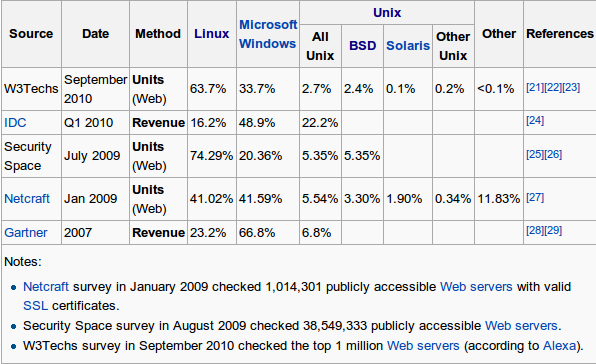
\includegraphics[width=10.0cm]{figs/servers-market.png}
\end{center}

\end{frame}

%%%%%%%%%%%%%%%%%%%%%%%%%%%%%%%%%%%%%%%%%%%%%%%%%%%%%%%%%%%%%%%%%%%%%%%

\begin{frame}
\frametitle{Compañías de hosting más fiables}

\begin{center}
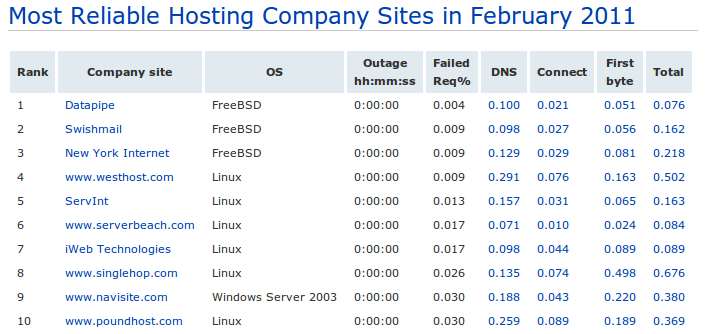
\includegraphics[width=11.5cm]{figs/netcraft.png}
\end{center}

\end{frame}

%%%%%%%%%%%%%%%%%%%%%%%%%%%%%%%%%%%%%%%%%%%%%%%%%%%%%%%%%%%%%%%%%%%%%%%

\subsection{¿No hay desventajas?}
\begin{frame}
\frametitle{Desventajas}

\pause

\begin{itemize}
\item Necesidad de técnicos especializados (la gente se forma con SO privativos)
\item Interfaces visuales (suelen ser privativos)
\item No siempre hay soporte para todo tipo de hardware (patentes, drivers y especificaciones privativas).
\item Suele ser necesario hacer \textit{advocacy} y plantear migraciones
\item ¿Mayor mercado laboral en sistemas privativos? (depende del sector)
\end{itemize}
\end{frame}

%%%%%%%%%%%%%%%%%%%%%%%%%%%%%%%%%%%%%%%%%%%%%%%%%%%%%%%%%%%%%%%%%%%%%%%

\begin{frame}
\frametitle{¿Y qué hay de las GUIs?}

\pause

\begin{itemize}
\item Muchas distros traen GUIs o herramientas visuales propias. 
\item Son útiles y facilitan las tareas, sobre todo para sysadmins noveles.
	\begin{itemize}
	\item Suelen ser propietarias
	\item O nos hacen dependientes de una distro en concreto
	\item A veces poseen oscuros detalles en la forma de gestionar los recursos
	\end{itemize}
\item Nosotros veremos siempre en las tecnologías y métodos subyacentes
\item Estos suelen ser comunes a todas las distros, incluso a todos los Unixes.
\item La configuración manual es mejor: más rápida, más flexible, más fiable, más potente y más \textit{scriptable}.
\end{itemize}
\end{frame}



%%%%%%%%%%%%%%%%%%%%%%%%%%%%%%%%%%%%%%%%%%%%%%%%%%%%%%%%%%%%%%%%%%%%%%%

\begin{frame}
\frametitle{¿Es gratis el software libre? Algunos consejos}

\pause

\begin{itemize}
\item La gratuidad NO es el punto fuerte del software libre
\item Insistir en la gratuidad supone minusvalorar el resto de ventajas (y es injusto para la gente que lo crea y lo mantiene).
\item No comiences hablándoles de dinero a los que toman decisiones.
\item No hablar del FLOSS en abstracto (``Linux es mejor''): estudia costes de migración y trata de cubrir necesidades concretas que no están cubiertas o mejorar lo que hay.
\item No seas impaciente: deja que el software libre crezca con los clientes, introduciendo mejoras de forma progresiva.
\end{itemize}
\end{frame}


%%%%%%%%%%%%%%%%%%%%%%%%%%%%%%%%%%%%%%%%%%%%%%%%%%%%%%%%%%%%%%%%%%%%%%%
\section{Tareas esenciales de un administrador de sistemas}
%%%%%%%%%%%%%%%%%%%%%%%%%%%%%%%%%%%%%%%%%%%%%%%%%%%%%%%%%%%%%%%%%%%%%%%

\begin{frame}
\frametitle{¿Qué es un administrador de sistemas?}

\vspace{-1cm}

\begin{block}{}
``\textit{Un \textbf{administrador de sistemas} es aquel profesional que tiene la responsabilidad de ejecutar, mantener, operar y asegurar el correcto funcionamiento de un sistema informático y/o una red de ordenadores.}'' (Wikipedia)
\end{block}

\medskip

Tambien llamado \alert{sysadmin}, debe demostrar una mezcla de:

\begin{itemize}
\item \alert{cualidades técnicas} 
\item \alert{responsabilidad} 
\item \alert{trabajo en equipo}
\end{itemize}

\end{frame}

%%%%%%%%%%%%%%%%%%%%%%%%%%%%%%%%%%%%%%%%%%%%%%%%%%%%%%%%%%%%%%%%%%%%%%%

\begin{frame}
\frametitle{Tareas esenciales de la administración de sistemas}

\begin{itemize}
\item Instalación, soporte y mantenimiento de servidores o de otros sistemas informáticos.
\item \textit{Scripting} o programación ligera. 
\item Gestión de proyectos en proyectos relacionados con sistemas. 
\item Supervisión y formación de operadores. 
\item Mantenimiento: monitorización del sistema, ejecutar backups, actualizar software, añadir y retirar hardware...
\item Creación, organización y mantenimiento de la documentación.
\item Soporte a usuarios.
\end{itemize}

\small

Todas estas tareas no necesariamente las lleva a cabo una sola persona. Pero al menos una persona debe conocerlas y asegurarse de que alguien las hace.

\end{frame}


%%%%%%%%%%%%%%%%%%%%%%%%%%%%%%%%%%%%%%%%%%%%%%%%%%%%%%%%%%%%%%%%%%%%%%%

\begin{frame}
\frametitle{Cualidades}

\begin{itemize}
\item Tenacidad para resolver problemas (incluso obsesivos).
\item Deseo genuino de ayudar a la gente.
\item Buena resistencia a trabajar bajo presión (entornos en producción).
\item Modestia (su trabajo no suele ser reconocido)
\item Los sysadmins suelen considerar divertido lo que hacen \textit{por sí mismo}.
\end{itemize}
\end{frame}

%%%%%%%%%%%%%%%%%%%%%%%%%%%%%%%%%%%%%%%%%%%%%%%%%%%%%%%%%%%%%%%%%%%%%%%

\begin{frame}
\frametitle{Habilidades, formación}

\begin{itemize}
\item La administración de sistemas implica más cambios de contexto en un solo día que la mayoría de trabajos en un año.
\item Un sysadmin necesita habilidad para organizarse y gestionar su tiempo eficientemente.
\item Habilidad para mantener felices a los usuarios en una situación \textit{win-win}.
\item El ``queme'' en el trabajo de un sysadmin es creciente. La mayoría de los administradores duran solo unos cuantos años.
\item A diferencia de otras profesiones, no existe una única vía para convertirse en sysadmin.
\end{itemize}
\end{frame}

%%%%%%%%%%%%%%%%%%%%%%%%%%%%%%%%%%%%%%%%%%%%%%%%%%%%%%%%%%%%%%%%%%%%%%%

\begin{frame}
\frametitle{Tipos de sysadmin}

\begin{itemize}
\item senior
\item operador
\item soporte técnico 
\item administrador de base de datos (DBA)
\item administrador de seguridad
\item administrador web
\item DevOps
\end{itemize}
\end{frame}

%%%%%%%%%%%%%%%%%%%%%%%%%%%%%%%%%%%%%%%%%%%%%%%%%%%%%%%%%%%%%%%%%%%%%%%

\begin{frame}
\frametitle{Discusión}

\begin{itemize}
\item ¿Qué está mejor valorado: un sysadmin o un developer?
\item ¿Se innova más en el desarrollo o en sistemas?
\item ¿Cualquiera puede ser sysadmin? ¿Todos somos un poco sysadmins?
\end{itemize}
\end{frame}

%%%%%%%%%%%%%%%%%%%%%%%%%%%%%%%%%%%%%%%%%%%%%%%%%%%%%%%%%%%%%%%%%%%%%%%
\subsection{Políticas y procedimientos}
%%%%%%%%%%%%%%%%%%%%%%%%%%%%%%%%%%%%%%%%%%%%%%%%%%%%%%%%%%%%%%%%%%%%%%%

\begin{frame}
\frametitle{Documentación}

\begin{itemize}
\item Lo último que quiere hacer un sysadmin es crear o mantener documentación. 
\item Tarea ardua y poco valorada. 
\item Tampoco suelen querer aprender herramientas como LaTeX, SGML o groff.
\end{itemize}

\end{frame}

%%%%%%%%%%%%%%%%%%%%%%%%%%%%%%%%%%%%%%%%%%%%%%%%%%%%%%%%%%%%%%%%%%%%%%%

\begin{frame}
\frametitle{Importancia de documentar}

\begin{itemize}
\item La documentación ayuda a la reproducibilidad. 
\item La documentación ahorra tiempo. 
\item La documentación facilitan el aprendizaje de nuevos administradores (algo que beneficia a todos). 
\item Lo principal: la documentación mejora la inteligibilidad de un sistema y permite que
	las modificaciones se hagan de un modo consistente.
\end{itemize}

\end{frame}

%%%%%%%%%%%%%%%%%%%%%%%%%%%%%%%%%%%%%%%%%%%%%%%%%%%%%%%%%%%%%%%%%%%%%%%

\begin{frame}
\frametitle{Importancia de documentar}

\begin{itemize}
\item Escribe documentos cortos: de una página que cubran un solo tema.
\item La documentación local debe guardarse en un solo punto bien definido y conocido (wiki, repo, sección de páginas \texttt{man}...).
\item Los propios ficheros de configuración deben comentarse.
\item Los wikis son ideales para documentar políticas y procedimientos del equipo de sistemas.
\item Recuerda: antes de automatizar, hay que haberlo hecho al menos una vez manualmente.
\end{itemize}

\end{frame}


%%%%%%%%%%%%%%%%%%%%%%%%%%%%%%%%%%%%%%%%%%%%%%%%%%%%%%%%%%%%%%%%%%%%%%%

\begin{frame}
\frametitle{Recursos documentales}

\begin{itemize}
\item Páginas \texttt{man}: tradicional doc. online.
	\begin{itemize}
	\item Están organizadas por secciones. 
	\item Una misma orden puede estar en varias secciones.
	\item No son howtos. 
	\end{itemize}
\item GNU Texinfo (reemplazo del formateador nroff --privativo-- usado en AT\&T). Hoy tiene poco sentido, pero GNU las sigue apoyando. 
\item Guías y documentación específica de cada sistema (ej. \textit{FreeBSD Handbook} o \texttt{docs.sun.com})
\item Documentación específica del paquete: (ej. \texttt{/usr/share/doc})
\item Libros en papel (O'Reilly)
\item Linux Documentation Project
\item RFCs
\end{itemize}

\end{frame}


%%%%%%%%%%%%%%%%%%%%%%%%%%%%%%%%%%%%%%%%%%%%%%%%%%%%%%%%%%%%%%%%%%%%%%%

\begin{frame}
\frametitle{Procedimientos}

Algunas tareas comunes que suelen necesitar procedimientos:

\begin{itemize}
\item Añadir un \textit{host}
\item Añadir un usuario
\item Configurar los backups para una nueva máquina
\item Securizar una nueva máquina
\item Actualizar el sistema operativo
\item Hacer respaldo y restauración de datos
\item Ejecutar apagados de emergencia
\end{itemize}
\end{frame}

%%%%%%%%%%%%%%%%%%%%%%%%%%%%%%%%%%%%%%%%%%%%%%%%%%%%%%%%%%%%%%%%%%%%%%%

\begin{frame}
\frametitle{Políticas}

Políticas habituales:

\begin{itemize}
\item Políticas de seguridad
\item Políticas para los administradores (login, sudo, pfexec...)
\item Acceso y políticas de usuario
\item Política de privacidad
\item Cuestiones legales: copyright (licencias y datos almacenados), cifrado, protección de datos personales\dots
\end{itemize}
\end{frame}


%%%%%%%%%%%%%%%%%%%%%%%%%%%%%%%%%%%%%%%%%%%%%%%%%%%%%%%%%%%%%%%%%%%%%%%

\subsection{Sistemas de seguimiento de incidencias}

\begin{frame}
\frametitle{Sistemas de seguimiento de incidencias}

\begin{itemize}
\item Software para crear, actualizar y resolver listas de incidencias. Similar a una 
"bugtracker". 
\item Contiene una base de conocimientos con soluciones a problemas comunes: recurso de valor incalculable para el personal administrador de sistemas. 
\item \alert{Ticket/incidencia:} una ficha que contiene información sobre las intervenciones de soporte realizadas por el personal técnico. 
\item Trac (python), RT (Perl), Redmine (RoR), OTRS, Mantis...: \url{http://en.wikipedia.org/wiki/Comparison_of_issue_tracking_systems}
\end{itemize}
\end{frame}

%%%%%%%%%%%%%%%%%%%%%%%%%%%%%%%%%%%%%%%%%%%%%%%%%%%%%%%%%%%%%%%%%%%%%%%


\begin{frame}
\frametitle{Funciones comunes de un sistema de gestión de incidencias}

Los responsables de proyecto pueden extraer valiosa información de alto nivel como:

\begin{itemize}
\item El número de tickets abiertos 
\item El tiempo medio en cerrarse un ticket
\item La productividad de los sysadmins
\item El porcentaje de tickets no resueltos
\item Posibles desequilibrios en la distribución de la carga de trabajo

\end{itemize}
\end{frame}


%%%%%%%%%%%%%%%%%%%%%%%%%%%%%%%%%%%%%%%%%%%%%%%%%%%%%%%%%%%%%%%%%%%%%%%

\begin{frame}
\frametitle{Flujo}

\begin{itemize}
\item El usuario (o el \textit{helpdesk}) reporta un problema.
\item El operador verifica que el problema es real y no solo una impresión.
\item EL operador se asegura de obtener suficiente información sobre el problema por parte del usuario.
\item La incidencia se asigna a la persona adecuada, que la marca como resuelta/cerrada/wontfix/feedback

\end{itemize}
\end{frame}

%%%%%%%%%%%%%%%%%%%%%%%%%%%%%%%%%%%%%%%%%%%%%%%%%%%%%%%%%%%%%%%%%%%%%%%

\begin{frame}
\frametitle{Un gestor avanzado de incidencias: Redmine}

Principales características:
\begin{itemize}
\item Soporte multi-proyecto
\item ACLs: acceso basado en roles muy flexibles. 
\item Wiki por proyecto
\item Integración con SCM (SVN, CVS, Git, Mercurial, Bazaar y Darcs)
\item Soporte para auto-registro
\item Diagrama de Gantt y calendario
\item Feeds y notificación por e-mail.
\end{itemize}
\end{frame}


%%%%%%%%%%%%%%%%%%%%%%%%%%%%%%%%%%%%%%%%%%%%%%%%%%%%%%%%%%%%%%%%%%%%%%%
\section{Asociaciones y organizaciones profesionales}
%%%%%%%%%%%%%%%%%%%%%%%%%%%%%%%%%%%%%%%%%%%%%%%%%%%%%%%%%%%%%%%%%%%%%%%

\subsection{SAGE}
\begin{frame}
\frametitle{SAGE}

\begin{itemize}
\item Es la primera organización internacional para sysadmins.
\item Es un grupo de interés dentro de Usenix.
\item Promueve la administración de sistemas como profesión y patrocina conferencias y programas informales.
\item Organiza el mayor evento para sysadmins: la conferencia USENIX LISA (Large Installation System Administration) en otoño.
\item SAGE se enfoca más a la investigación.
\end{itemize}
\end{frame}

%%%%%%%%%%%%%%%%%%%%%%%%%%%%%%%%%%%%%%%%%%%%%%%%%%%%%%%%%%%%%%%%%%%%%%%

\subsection{LOPSA}
\begin{frame}
\frametitle{LOPSA}

\begin{itemize}
\item LOPSA, League of Professional System Administrators.
\item Se creó en 2005 por parte de algunos miembros de SAGE. 
\item Misión: 
	\begin{itemize}
	\item promover la práctica de la administración de sistemas; 
	\item apoyar, reconocer, educar y alentar a los sysadmins; 	
 	\item servir al público por medio de la educación y divulgación en temas relacionados con la administración de sistemas.
	\end{itemize}
\item LOPSA busca brindar apoyo legislativo a los temas que afectan a la profesión.
\item SAGE y LOPSA cooperar en objetivos comunes, como el Código de Ética y la conferencia LISA.

\end{itemize}
\end{frame}



%%%%%%%%%%%%%%%%%%%%%%%%%%%%%%%%%%%%%%%%%%%%%%%%%%%%%%%%%%%%%%%%%%%%%%%

\subsection{Código ético}
\begin{frame}
\frametitle{Código ético (1)}

LOPSA, USENIX y SAGE animan a que todo administrador se guía por un código ético:  

\begin{itemize}
\item Profesionalidad
\item Integridad personal
\item Privacidad
\item Leyes y políticas
\item Comunicación
\end{itemize}
\end{frame}

%%%%%%%%%%%%%%%%%%%%%%%%%%%%%%%%%%%%%%%%%%%%%%%%%%%%%%%%%%%%%%%%%%%%%%%

\begin{frame}
\frametitle{Código ético (2)}

\begin{itemize}
\item Integridad de sistema
\item Educación
\item Responsabilidad social
\item Responsabilidad ética
\end{itemize}

\url{http://lopsa.org/CodeOfEthics}

\end{frame}

%%%%%%%%%%%%%%%%%%%%%%%%%%%%%%%%%%%%%%%%%%%%%%%%%%%%%%%%%%%%%%%%%%%%%%%

\section{DevOps}
\subsection{Contexto}

\begin{frame}
  \frametitle{Contexto}
  \begin{itemize}
    \item Los departamentos de sistemas y desarrollo trabajan aislados
% Los desarrolladores dan el código y los requisitos pero cuando algo falla dicen "en mi local funciona"
% Los desarrolladores nos piden instalar algo no paquetizado y los sysadmins dicen "no!"
    \item Cada uno de los departamentos considera que hace los correcto para el negocio
% Seguro que, analizado de forma aislada, ambos tienen razón
    \item Los desarrolladores no tienen ``conciencia'' de sistemas
% No saben del impacto en los sistemas; ellos tienen herramientas locales para el desarrollo
    \item Ambos departamentos son imprescindibles para el negocio
% Los desarrolladores implementan los requisitos funcionales
% Los sysadmins implementan seguridad, estabilidad y rendimiento
% Están condenados a entenderse porque son objetivos que entran en conflicto
    \item Aparecen las metodologías ágiles de desarrollo: muchos cambios muy pequeños
% Los cambios son los que generan problemas de seguridad, rendimiento y estabilidad
% Los sysadmins a menudo intentan no hacer cambios y los desarrolladores necesitan muchos cambios
  \end{itemize}
\end{frame}

%%%%%%%%%%%%%%%%%%%%%%%%%%%%%%%%%%%%%%%%%%%%%%%%%%%%%%%%%%%%%%%%%%%%%%%

\begin{frame}
  \frametitle{Necesidades}
  \begin{itemize}
    \item Romper las barreras entre los departamentos de sistemas y desarrollo.
    \item Implantar metodologías ágiles en sistemas.
    \item Usar frameworks de automatización: puppet, chef, cfengine...
    \item Mecanismos de comunicación efectivos entre ambos departamentos.
    \item Sistemas ha de estar involucrado en el diseño de la aplicación desde el principio.
  \end{itemize}

  \begin{center}
    \item El objetivo final es permitir al negocio que reaccione tan rápido, eficiente y fiable como marca el mercado
  \end{center}
\end{frame}

%%%%%%%%%%%%%%%%%%%%%%%%%%%%%%%%%%%%%%%%%%%%%%%%%%%%%%%%%%%%%%%%%%%%%%%

\subsection{Qué es DevOps}

\begin{frame}
  \frametitle{Qué es DevOps}
  \begin{block}{}
    Filosofía apoyada en procedimientos, herramientas y métodos para permitir una colaboración efectiva entre sysadmins y developers que posibiliten eficientemente el objetivo del negocio.
  \end{block}
  \begin{itemize}
    \item No es un perfil de empleado
% Nadie dice voy a contratar a un Scrum o ITIL, sino un desarrollador que comparta esas metodologías
    \item No es una nueva forma de llamar a los sysadmins
    \item No se trata de superponer ni menospreciar puestos; al contrario
% No es cosa de los desarrolladores para librarse de los sysadmins
% No es de los sysadmins para librarse de los desarrolladoras
% Son las dos cosas a la vez
    \item No es un problema tecnológico, es un problema del negocio
  \end{itemize}
\end{frame}

%%%%%%%%%%%%%%%%%%%%%%%%%%%%%%%%%%%%%%%%%%%%%%%%%%%%%%%%%%%%%%%%%%%%%%%

\begin{frame}
\frametitle{Referencias}

\begin{itemize}
\item Nemeth, Snyder, Hein \textit{UNIX and Linux System Administration Handbook}
\item Limoncelli, Thomas A. \textit{Time Management for System Administrators} 
\end{itemize}

\end{frame}

%%%%%%%%%%%%%%%%%%%%%%%%%%%%%%%%%%%%%%%%%%%%%%%%%%%%%%%%%%%%%%%%%%%%%%%

\frame{
\maketitle
\begin{center}

\includegraphics[width=6cm]{format/gsyc-urjc}
\end{center}
}


\end{document}

